\chapter{First Steps on MFC implementation}

\section{Model Following Control}
\label{sec:MFC}

\subsection{Overview}

The Model Following Control (MFC) Loop is described FIGURE.\ref{fig:MFC Control Loop}.

\begin{figure}[htbp]
    \centering
    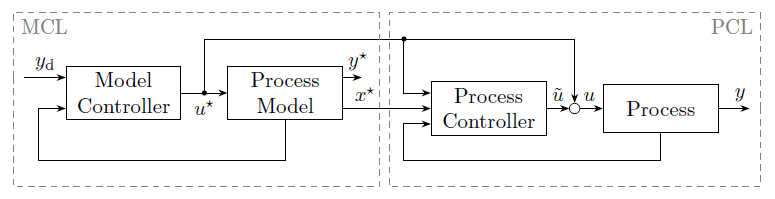
\includegraphics[width=1\linewidth]{imgs/section1/MFC_scheme.PNG}
    \caption{Model Following control block diagram with model control loop process and control loop}
    \label{fig:MFC Control Loop}
\end{figure}

One can see that the model following control consist into the creation of two loops : the model control loop (MCL) and the process control loop (PCL). The first one is used to fulfill a nominal control based on the model of the theoretical plant to be controlled. It provides a nominal output \(y^*\), nominal states \(x^*\) and a nominal control input \(u^*\). The nominal states are used as reference for the PCL that will compensate the perturbations with the control input \(\tilde{u}\). Thus the control is the addition of \(\tilde{u}\) and \(u^*\) used as a feedforward. The MCL presents no uncertainties such that the model controller can be tuned regarding the nominal performance of tracking the desired
output \(y_d\). 

This controller architecture is based on the work done in \textbf{CITER LA THESE MFC}


%_________________________________________________________________________________________%
\subsection{System Class}


We consider a non linear SISO system into the flat form :

\begin{equation}
\label{eq:flat_sys}
\left\{
\begin{aligned}
  \dot{\eta} &= f_0(\eta, \xi) \\
  \dot{\xi} &= A\xi + B\big(a(\xi,\eta) + b(\xi,\eta)u + \phi(\xi,\eta) + \delta\big) \\
  y &= C\xi
\end{aligned}
\right.
\end{equation}



where \( \eta(t) \in \mathbb{D}_\eta \subseteq \mathbb{R}^{n - r} \) and \( \xi(t) \in \mathbb{D}_\xi \subseteq \mathbb{R}^r \) denote the internal and external states, respectively.  
The output is \( y(t) \in \mathbb{R} \) and \( u(t) \in \mathbb{R} \) denotes the input. The relative degree is \( 1 \leq r \leq n \). The matrices \( A \), \( B \), and \( C \) are given by

\begin{equation}
A = 
\begin{bmatrix}
0 & 1 & 0 & \cdots & 0 \\
0 & 0 & 1 & \cdots & 0 \\
\vdots & \vdots & \ddots & \ddots & \vdots \\
0 & 0 & \cdots & 0 & 1 \\
0 & 0 & \cdots & 0 & 0 
\end{bmatrix}
\in \mathbb{R}^{n \times n}, \quad
B = 
\begin{bmatrix}
0 \\
0 \\
\vdots \\
0 \\
1 
\end{bmatrix}
\in \mathbb{R}^n, \quad
C = 
\begin{bmatrix}
1 & 0 & \cdots & 0 
\end{bmatrix}
\in \mathbb{R}^{1 \times n} 
\end{equation}

In our case, we will assume that there are no internal dynamics i.e. \( r = n\), the system \ref{eq:flat_sys} becomes : 

\begin{equation}
\label{eq:flat_sys_reduced}
\left\{
\begin{aligned}
  \dot{\xi} &= A\xi + B\big(a(\xi) + b(\xi)u + \phi(\xi) + \delta\big) \\
  y &= C\xi
\end{aligned}
\right.
\end{equation}

We will assume that the unknown model uncertainty \(\phi: \mathbb{D}_{\xi} \times \mathbb{D}_{\eta} \rightarrow \mathbb{R}\) to be (at least locally) Lipschitz in the domain of interest and to be bounded in the origin, i.e., \(|\phi(0,0)| \leq d_{\phi}\) with \(0 \leq d_{\phi} < \infty\). The external disturbance \(\delta(t) \in \mathbb{R}\) is assumed to be piecewise continuous and bounded by

\begin{equation}
     |\delta(t)| \leq d \quad \forall t \in [0, \infty) 
\end{equation}

with constant \(0 \leq d < \infty\). These assumptions are required to prove the stability of the dynamics.

We will see in the further points that the crane system model is non-linear and of form : 

\begin{align}
    \dot{x} &= f(x) + g(x)u + \Phi(x) + g_\delta(x)\delta_x \\
    y &= h(x)
\end{align}

However it can be transformed into \ref{eq:flat_sys_reduced} by computing a feedback linerarization. Respectivly \(x(t) \in \mathbb{R}^{n} \), \(u(t) \in \mathbb{R}\) and \(y(t)\ \in \mathbb{R}\) denote the states, the inut and the output. the external disturbances are assumed to be bounded and \(f: \mathbb{R}^n \rightarrow \mathbb{R}^n\), \(g: \mathbb{R}^n \rightarrow \mathbb{R}^n\), \(g_\delta: \mathbb{R}^n \rightarrow \mathbb{R}^n\), \(h: \mathbb{R}^n \rightarrow \mathbb{R}\) and \(\Phi: \mathbb{R}^n \rightarrow \mathbb{R}^n\) are sufficiently smooth function. Only \(\Phi(.)\) is unknown.
 
We apply the transformation given by :

\begin{equation}
\begin{bmatrix}
\xi_1 \\
\xi_2 \\
\xi_3 \\
\vdots \\
\xi_n \\
\end{bmatrix}
=
T(x)
=
\begin{bmatrix}
h(x) \\
\mathcal{L}_f h(x) \\
\mathcal{L}_f^2 h(x) \\
\vdots \\
\mathcal{L}_f^{n-1} h(x) \\
\end{bmatrix}
\end{equation}

where \( T(x) \) is a diffeomorphism \textbf{cite KHALIL}. If the restrictive conditions


\begin{equation}
\left\{
\begin{aligned}
\mathcal{L}_g \mathcal{L}_f^i h(x) &= 0, \quad & 0 \leq i \leq n-2, \\
\mathcal{L}_g \mathcal{L}_f^{n-1} h(x) &\neq 0, \\
\mathcal{L}_{\Phi} \mathcal{L}_f^i h(x) &= 0, \quad & 0 \leq i \leq n-2, \\
\mathcal{L}_{g\delta} \mathcal{L}_f^i h(x) &= 0, \quad & 0 \leq i \leq n-2.
\end{aligned}
\right.
\end{equation}


are satisfied and \( k_{\delta} = \mathcal{L}_{g\delta} \mathcal{L}_f^{r-1} h(x) \) is a constant independent of \( x \), then the transformed system is of the form \ref{eq:flat_sys_reduced} with

\begin{align}
a(\xi) &= \mathcal{L}_f^r h(x)\big|_{x=T^{-1}(\xi)}, & b(\xi) &= \mathcal{L}_g \mathcal{L}_f^{r-1} h(x)\big|_{x=T^{-1}(\xi)}, \\
\phi(\xi) &= \mathcal{L}_{\Phi} \mathcal{L}_f^{r-1} h(x)\big|_{x=T^{-1}(\xi)}, & \delta &= \mathcal{L}_{g\delta} \mathcal{L}_f^{r-1} h(x) \delta_x = k_{\delta} \delta_x.
\end{align}

The goal is now to ensure the convergence of the tracking reference \(y_d(t) \in \mathbb{R}\) i.e. : 
\[\lim\limits_{x \to +\infty} \left( y(t) - y_d(t) \right) = 0\]
while ensuring the boundness of \(\xi\). We need \(y_d\) to be n-times differentiable with all of its derivatives bounded.


%_________________________________________________________________________________________%
\subsection{Model Control Design}

An analysis of the control loop dynamics can be carried out in two stages. First, we consider the Model Control Loop (MCL), which is a replica of system \ref{eq:flat_sys_reduced}, excluding external disturbances \(\delta\) and model uncertainties \(\phi(\xi)\), and is described by:

\begin{equation}
\label{eq:MCL_open_loop}
  \dot{\xi^*} = A\xi^* + B\big(a(\xi^*) + b(\xi^*)u^* \big)
\end{equation}

It is observed that the input signal is decomposed as \(u = \tilde{u} + u^*\), where \(u^*\) denotes the output of the MCL and \(\tilde{u}\) the output of the process control loop. The overall dynamics of the Model-Following Control (MFC) framework are thus governed by both the model dynamics and the error dynamics, which are derived from the discrepancy between the model and the actual process. The error states are defined as \(\tilde{\xi} = \xi - \xi^*\), and the open-loop dynamics of the MFC are given by:

\begin{align}
\dot{\xi}^* &= A\xi^* + B \left( a(\xi^*) + b(\xi^*) u^* \right) \\
\dot{\tilde{\xi}} &= A\tilde{\xi} + B \left( \tilde{a}(\xi^*, \tilde{\xi}, u^*) + b(\xi^* + \tilde{\xi}) \tilde{u} + \phi(\xi^* + \tilde{\xi}) + \delta \right)
\end{align}

where

\begin{align}
\tilde{a}(\xi^*, \tilde{\xi}, u^*) &= a(\xi^* + \tilde{\xi}) - a(\xi^*) + \left( b(\xi^* + \tilde{\xi}) - b(\xi^*) \right) u^*
\end{align}

We now aim to design a controller for the MFC that ensures closed-loop stability. Following the approach proposed by \textbf{CITE THESE MFC}, a (partial) feedback linearization is applied to the MCL, defined by:

\begin{equation}
\label{eq:MCL_control_law}
u^* = -\frac{a(\xi^*) + v^*}{b(\xi^*)}
\end{equation}

This compensates for the nonlinearities in the model dynamics and introduces the new control input \(v^*\). The design of \(v^*\) is based on the error dynamics within the MCL. To this end, we define the model tracking errors \(\tilde{\xi}^* = \xi^* - \xi_d\), representing the deviation between the model and desired states. The associated error dynamics are given by:

\begin{align}
\dot{\tilde{\xi}}^* &= A\tilde{\xi}^* + B(v^* - y_d^{(r)})
\end{align}

The new input \(v^*\) is chosen as:

\begin{equation}
v^* = y_d^{(r)} + K\tilde{\xi}^*
\end{equation}

where \(K = [-\alpha_0, -\alpha_1, \ldots, -\alpha_{r-1}] \in \mathbb{R}^{1 \times r}\) is selected such that the matrix \(A + BK\) is Hurwitz. Consequently, the closed-loop dynamics of the MCL become:

\begin{align}
\dot{\tilde{\xi}}^* &= (A + BK)\tilde{\xi}^*
\end{align}

To ensure the stability of the model dynamics, we consider the quadratic Lyapunov function \(V(\tilde{\xi}^*) = \tilde{\xi}^{*\top} P \tilde{\xi}^*\), where \(P\) is a symmetric positive definite matrix satisfying the Lyapunov equation:

\begin{equation}
\label{eq:Moreno}
(A + BK)^\top P + P(A + BK) = -Q = -I
\end{equation}

with \(I\) denoting the identity matrix of suitable dimension. Since \(A + BK\) is Hurwitz by construction, the solution \(P\) exists and is unique. Although the right-hand side of \ref{eq:Moreno} allows for a general choice of symmetric positive definite matrices \(Q\), the selection \(Q = I\) is particularly advantageous as it maximizes the ratio \(\lambda_{\min}(Q) \lambda_{\max}^{-1}(P)\).

The MCL dynamics are proven to be stable in \textbf{CITE THESE MFC}. Now can can apply the same principle to the process control loop.

%_________________________________________________________________________________________%
\subsection{Process Control Loop}

The process control loop is design to counter the perturbations and model uncertainties. The design method to assure robustness is the high-control gain approach. This sort of feed-back controller presents real assets to assure the origin stabilization, set-point tracking control or trajectory tracking control. But it comes at a price in terms of performance showing a peaking phenomenon due to the high input effort easily computed from the high-gains. We will see in the following simulation and test that the architecture of the MFC mitigate these behavior be choosing the right initial conditions.

The desired output trajectory`\(y_d(t) \in \mathbb{R}\) is assumed to be at least n-times continuously differentiable. The desired external states \(\xi_d(t) \in \mathbb{D}_{\xi_d}  \subseteq \mathbb{R}^n\) are generated by 

\begin{equation}
    \dot{\xi_d} = A\xi_d + By_d^{(n)}
\end{equation}

We can recall the MCL control law \ref{eq:MCL_control_law} given by 
\begin{equation}
    u^* = \frac{-a(\xi^*) + y_d^{(n)} + K(\xi^* - \xi_d)}{b(\xi^*)}
\end{equation}

The open-loop error dynamics are given by

\begin{align}
\dot{\tilde{\xi}} &= A\tilde{\xi} + B\left(\tilde{a}(\xi^*, \tilde{\xi}, u^*) + b(\tilde{\xi}^* + \tilde{\xi}) \tilde{u} + \phi(\tilde{\xi}^* + \tilde{\xi}) + \delta\right)
\end{align}


Based on what we have implemented in the MCL, the design of the process controller will also be a feedback linearizing control law 

\begin{equation}
\tilde{u} = \frac{-\tilde{a}(\xi^*, \tilde{\xi}, u^*) + \tilde{K}\tilde{\xi}}{b(\xi^* + \xi)}
\end{equation}

where the feedback matrix is chosen as

\begin{equation}
\tilde{K} = KD^{-1}\varepsilon^{-1}
\end{equation}

with \(D = \text{diag}(\varepsilon^{r-1}, \varepsilon^{r-2}, \ldots, 1)\) and \(0 < \varepsilon < 1\) is a time scaling parameter \(\epsilon\) satisfying \(\epsilon=\frac{dt}{d\tau}\). Applying the control law to the external error dynamics yields

\begin{equation}
\dot{\tilde{\xi}} = (A + BKD^{-1}\epsilon^{-1})\tilde{\xi} + B(\phi(\xi^* + \tilde{\xi}) + \delta)
\end{equation}

We proceed the time scaling change of variable : 

\begin{equation}
    \zeta = D^{-1}\tilde{\xi}
\end{equation}

The closed-loop overall dynamics of the MFC scheme for set-point and trajectory tracking are given by

\begin{align}
\label{eq:The closed-loop overall dynamics of the MFC}
\dot{\tilde{\xi}}^* &= (A + BK)\tilde{\xi}^* \\
\varepsilon\dot{\zeta} &= (A + BK)\zeta + \varepsilon B \left(\phi(\xi_d + \tilde{\xi}^* + D\zeta) + \delta\right).
\end{align}

Observe that if \( A + BK \) is Hurwitz, the eigenvalues of the error dynamics (without time-scaling) can be shifted arbitrarily far to the left of the imaginary axis as \( \epsilon \rightarrow 0 \). This implies that, theoretically, the error dynamics can be made to converge arbitrarily quickly. However, achieving this may necessitate a significantly large control effort. Additionally, a small \( \epsilon \) enhances robustness against model uncertainties \( \phi(\xi) \), alongside accelerating the error dynamics of the PCL.


The dynamics of \ref{eq:The closed-loop overall dynamics of the MFC} are proven to be stable in \textbf{CITE THESE MFC}.Now that we have constructed the complete MFC controller, we can start to implement it to the crane simulation. Therefore, one can notice that some modifications can be done to be freed of useless heavy function like \(\tilde{a}(.)\). That is what we will see in the next point with a simpler controller design.


%_________________________________________________________________________________________%
\subsection{A Simpler Design}




%_________________________________________________________________________________________%
%_________________________________________________________________________________________%
\section{Implementation on a Crane Simulation}

All of the control law has been defined, we can test its performances on a crane system but first, it will be run through a simulation on Matlab Simulink. The analysis is done in three situation, stabilizing on a setpoint and then setpoint and trajectory tracking. The goal is to observe the presence or not of the peaking phenomenon depending on the initial conditions of the Model Control Loop and we will verify just on the simulation the exact same behavior between the original MFC and the simpler design. 

%_________________________________________________________________________________________%
\subsection{Crane Model Overview}

\textbf{FAIRE SCHEMA DE LA GRUE}

This point is base on the work done in \textbf{CITE PAPIER CRANE}. 

The schematic setup of the three-dimensional overhead crane involves defining the trolley position and the load position relative to a fixed reference frame. The trolley position \(\boldsymbol{r}_{t}(t)\) is considered as a time-dependent function given by:

\begin{equation}
    \textbf{r}_t(t) = \begin{bmatrix}
        a(t) \; b(t) \; 0
    \end{bmatrix}^T
\end{equation}

where \(a(t)\) and \(b(t)\) are the position of the trolley in x and y direction. Then, thanks to the cardan angles of the pivot point \(\alpha\) and \(\beta\), one can express the position of the load, which will be the output of the system as \(\textbf{y}(t)\) given by :

\begin{equation}
    \textbf{y}(t) = \begin{bmatrix}
        a(t) + l(t)S_\beta \\
    b(t) + l(t)C_\beta S_\alpha \\
    -l(t)C_\beta C_\alpha
    \end{bmatrix}
\end{equation}

With the notations \(S_\gamma = sin(\gamma)\) and \(C_\gamma = cos(\gamma)\).

The goal is to find the dynamics of the generalized coordinates vector \(\boldsymbol{\theta} = \left[ \alpha \; \beta \right]^T\) to get the Newton-Euler equation of the load system. The velocity of the load is given by : 

\begin{equation}
    \dot{\mathbf{y}}(t) = \boldsymbol{J}_{l}(t) \cdot \dot{\boldsymbol{\theta}} + \underbrace{  \begin{bmatrix}
       \frac{\mathrm{d}a(t)}{\mathrm{d}t} + \frac{\mathrm{d}l(t)}{\mathrm{d}t} S_\beta \\
       \frac{\mathrm{d}b(t)}{\mathrm{d}t} + \frac{\mathrm{d}l(t)}{\mathrm{d}t} C_\beta S_\alpha \\
       -\frac{\mathrm{d}l(t)}{\mathrm{d}t} C_\beta C_\alpha
  \end{bmatrix}}_{\bar{\dot{\boldsymbol{y}}}(t)}
\end{equation}

Where \( \boldsymbol{J}_{l}(t)\) denotes the jacobian of the crane over the generalized coordinates and reads as : 

\begin{equation}
     \boldsymbol{J}_{l}(t) = \frac{\partial \boldsymbol{y}(t)}{\partial \boldsymbol{\theta}} = \begin{bmatrix}
         0                       & l(t)C_\beta \\
         l(t)C_\beta C_\alpha    & -l(t)S_\beta S_\alpha \\
         l(t)C_\beta S_\alpha    & l(t)S_\beta C_\alpha
     \end{bmatrix}
\end{equation}

Finally, the acceleration of the load is given by : 

\begin{equation}
    \ddot{\boldsymbol{y}}(t) = \boldsymbol{J}_{l}(t) \cdot \ddot{\boldsymbol{\theta}} + \underbrace{\frac{d\boldsymbol{J}_{l}(t)}{dt} \cdot \dot{\boldsymbol{\theta}} + \frac{d\bar{\dot{\boldsymbol{y}}}(t)}{dt}}_{\bar{\ddot{\boldsymbol{y}}}(t)}
\end{equation}

The mass matrix of the load with mass \(m\) is taken as punctual and given by :

\begin{equation}
    \boldsymbol{M} = \boldsymbol{I}_3 m
\end{equation}

\textbf{NE PAS OUBLIER DE DEFINIR LE Q}

where \(\boldsymbol{I}_3\) is the \(3 \times 3\) identity matrix. The Newton-Euler equation is applied to derive the equations of motion:

\begin{equation}  
\label{eq:Newton_Euler}
\boldsymbol{M} \boldsymbol{J}_{l}(t) \cdot \ddot{\boldsymbol{\theta}} = -\boldsymbol{M} \ddot{\boldsymbol{y}}(t) + \boldsymbol{q}_{e} + \boldsymbol{Q} \boldsymbol{q}_{r}
\end{equation}

where \(\boldsymbol{q}_{e}\) denotes the vector of external forces, primarily due to gravity. Hence \(\boldsymbol{Q}^T\boldsymbol{J}_{l}(t) = \boldsymbol{J}_{l}(t)^T\boldsymbol{Q}= 0\) and multiplying by \( \boldsymbol{J}_{l}(t)^T\), we eliminate the reaction forces \(\boldsymbol{q}_r\) in \ref{eq:Newton_Euler}, knowing that \(\boldsymbol{M} = \boldsymbol{I}_3m\) the equation of motion in generalized coordinates \(\boldsymbol{\theta}\) reads :

\begin{equation}
\label{eq:equation_of_motion_generalized_coordinates}
    m \cdot \boldsymbol{J}_{l}(t)^T\boldsymbol{J}_{l}(t)\cdot \ddot{\boldsymbol{\theta}} = - m \cdot\boldsymbol{J}_{l}(t)^T \: \bar{\ddot{\boldsymbol{y}}}(t) \; + \; m \cdot \boldsymbol{J}_{l}(t)^T\boldsymbol{g}
\end{equation}

Where \(\boldsymbol{g} = \begin{bmatrix} 0 & 0 & -g\end{bmatrix}^T\) denotes the gravity vector, and it is easy to remark that the equation \ref{eq:equation_of_motion_generalized_coordinates} is independent of the load mass \(m\). 

The input is be the same as in the simulation and the real crane experimentation, they will directly drive the \(\begin{bmatrix}\ddot{a}(t) & \ddot{b}(t) & \ddot{l}(t)\end{bmatrix}\) coordinates. Which gives us the complete dynamics of the crane plant system in the form of a non-linear vectorial second order differential equation : 


\begin{align}
\left\{ \begin{array}{ll}
\ddot{a}(t) &= u_1\\ 
\ddot{b}(t) &= u_2\\ 
\ddot{l}(t) &= u_3\\
\ddot{\alpha}(t) &= \frac{1}{l(t) C_{\beta}} \left(2 \dot{\alpha} \dot{\beta} S_{\beta} l(t) - 2 \dot{l}(t) \dot{\alpha} C_{\beta} - S_{\alpha} g - C_{\alpha} u_2\right) \\
\ddot{\beta}(t) &= \frac{1}{l(t)} \left(-C_{\alpha} S_{\beta} g - S_{\beta} C_{\beta} \dot{\alpha}^2 l(t) - 2 \dot{l}(t) \dot{\beta} + S_{\beta} S_{\alpha} u_2 - C_{\beta} u_1\right) \\
\end{array}
\right.
\end{align}

and the output : 

\begin{equation}
    \textbf{y}(t) = \begin{bmatrix}
        a(t) + l(t)S_\beta \\
        b(t) + l(t)C_\beta S_\alpha \\
        -l(t)C_\beta C_\alpha
    \end{bmatrix}
\end{equation}

We can now write this system into the normal form : 

\begin{align}
    \dot{x} &= f(x) + g(x)u \\
    h(x) &= y(x)
\end{align}

where : \begin{equation}
    x(t) = (x_i(t))_{1\le i\le 10} = \begin{pmatrix} a(t) & \dot{a}(t) & b(t) & \dot{b}(t) & l(t) & \dot{l}(t) & \alpha(t) & \dot{\alpha}(t) & \beta(t) & \dot{\beta}(t)\end{pmatrix}^T
\end{equation}

We have seen in \ref{sec:MFC} that a feedback linearization is needed to put the system into the MFC compatible form.

%_________________________________________________________________________________________%
\subsection{Feedback linearization and dynamic extension}

To get a flat system after the feedback linearization, an artificial increase of the relative degree is needed. We use a strategy of dynamic extension by writing : 

\begin{align}
    \ddot{\nu} &= w_3 \\
    u_3 &= \psi(x, \nu)
\end{align}

So that : \(\ddot{y}_3 = \nu\)

This new system gets a virtual input \(w_3\) so the new input vector is \(u_{ex} = \begin{pmatrix} u_1 & u_2 & w_3 \end{pmatrix}^T\) and \(u_3\) will be computed to assure : 
\begin{equation}
    \forall t \ge 0 \; , \quad \ddot{y}_3(t) - \nu(t) = 0
\end{equation}

This leads to a flat system of dimension \(n = 12\) that reads : 

\begin{equation}
\left\{
\begin{aligned}
  \dot{\xi} &= A\xi + B\big(a(\xi) + b(\xi)u) \\
  y &= C\xi
\end{aligned}
\right.
\end{equation}

We can remark that the term \( \phi(\xi) + \delta\) present in \ref{eq:flat_sys_reduced} isn't part of the feedback linearization. Indeed, it won't be there into the model control loop. But is practically present into the real system 

%_________________________________________________________________________________________%
\subsection{Matlab Control Loop}


%_________________________________________________________________________________________%
\subsection{Simulation Results}


%_________________________________________________________________________________________%
%_________________________________________________________________________________________%
\section{Real Crane Control}


%_________________________________________________________________________________________%
\subsection{System Overview}


%_________________________________________________________________________________________%
\subsection{D-Space}


%_________________________________________________________________________________________%
\subsection{Results}


%_________________________________________________________________________________________%
\section{Conclusion}








